%!TEX root = ../template.tex
%%%%%%%%%%%%%%%%%%%%%%%%%%%%%%%%%%%%%%%%%%%%%%%%%%%%%%%%%%%%%%%%%%%%
%% chapter4.tex
%% NOVA thesis document file
%%
%% Chapter with lots of dummy text
%%%%%%%%%%%%%%%%%%%%%%%%%%%%%%%%%%%%%%%%%%%%%%%%%%%%%%%%%%%%%%%%%%%%

\chapter{Diseño de una Red SD-WAN}
\label{cha:Diseño de una Red SD-WAN}

\section{Inversión para una SD-WAN} % (fold)
\label{sec:Inversión para una SD-WAN}

\section{Precios en una Red SD-WAN} % (fold)
\label{sec:Precios en una Red SD-WAN}

Una de las mayores motivaciones para el desarrollo de este proyecto es reducir el costo en OPEX que costarían los enlaces de los proveedores de servicio al trasladar los servicios de la empresa a la nube, ya que los costos de ancho de banda se reducirían notablemente al realizar esta migración con SD-WAN \textbf{la tabla 10.1} muestra una comparación aproximada de los costos de los enlaces WAN requeridos con y sin SD-WAN. 
\\
\\
Dichos costos son calculados tomando en cuenta los valores publicados por google para su aplicación de Gsuite, ya que el cliente entre otras cosas realizará reuniones a través de Google Meet, esto requiere 3.2MB de ancho de banda por participante.

\begin{table}[ht]
	\caption{Tabla de Precios  para la Implementación de una SW-WAN.}
	\label{tab:hla:results}
\centering
\begin{tabular}{lccccc}
	\toprule
	\multicolumn{1}{c}{\textbf{Tipo de Oficina}} 	& \textbf{Tienda}	& \textbf{Regional}	& \textbf{Oficina Regional}\\
	\midrule
\cite{Usuarios}~Promedio 		& 3 & 25 & 60	 \\
\cite{Sesiones}~de Video Simultáneas & 1& 8	& 20	\\
\cite{Trafico}~de Datos	& 5MB	& 10MB	& 20MB	\\
\cite{BW}~Servicio Actual		& 10& 7	& 14	 \\
\cite{BW}~Requerido	& 9MB	& 25MB	& 84MB	 \\
\cite{Costo}~Actual			& 221741	& 1260741	& 1803563	\\
\cite{Costo}~Mensual Red Legacy		& 221741	& 3607126	& 6782000 \\
\cite{Costo}~Mensual SD-WAN	& 221741	& 1842102	& 3972361\\
	\midrule
	\textbf{Total}			& \textbf{--}		& \textbf{--}		& \textbf{--} \\
	\bottomrule
\end{tabular}
\end{table}
Adicional al costo de los enlaces, el OPEX también se vería reducido al requerir menor tiempo de los recursos de IT en la administración de la red, ya que al automatizar las configuraciones y cambios la velocidad de aprovisionamiento se vería ampliamente mejorada y por tanto su costo sería menor.


\section{Costos para Implementación en Infraestructura Cloud} % (fold)
\label{sec:Costos para Implementación en Infraestructura Cloud}


\subsection{Amazon}

\textcolor{blue}{Amazon:} multinacional de comercio electrónico y servicios de computación en la nube, contiene cuatro modelos para compra de instancias en Cloud conocido como Amazon EC2.

\begin{itemize}
\item[•] \textbf{Baja Demanda:} \textit{"Con las instancias bajo demanda, paga por la capacidad informática por hora o por segundo, según las instancias que use. Ya no serán necesarios los contratos a largo plazo ni los pagos iniciales. Puede aumentar o reducir la capacidad informática en función de las exigencias de su aplicación y pagar únicamente la tarifa por hora específica de la instancia que use." En la \textbf{tabla 10.2} se observa algunos costos de baja demanda.}

\begin{table}[ht]
	\caption{Amazon EC2 Pricing.}
	\label{tab:hla:results}
\centering
\begin{tabular}{lccccc}
	\toprule
	\multicolumn{1}{c}{\textbf{vCPU}} 	& \textbf{ECU}	& \textbf{Memory (GiB)}	& \textbf{Instance Storage (GB)}
	& \textbf{Linux/UNIX Usage}\\
	\midrule
\cite{a1.medium}~1 		& N/A & 2GiB & EBS Only	& \$0.0255 per Hour \\
\cite{a1.large}~2 		& N/A & 4GiB & EBS Only & \$0.051 per Hour	\\
\cite{a1.xlarge}~4		& N/A & 4GiB & EBS Only & \$0.051 per Hour	\\
\cite{a1.2xlarge}~8 	& N/A & 16GiB & EBS Only & \$0.204 per Hour	\\
\cite{a1.4xlarge}~16	& N/A & 32GiB & EBS Only & \$0.408 per Hour	\\
\cite{t3.nano}~2		& N/A & 0.5GiB & EBS Only & \$0.0052 per Hour	\\
\cite{t3.micro}~2   	& N/A & 1GiB & EBS Only & \$0.0104 per Hour	\\
	\midrule
	\textbf{Total}			& \textbf{--}		& \textbf{--}		& \textbf{--} \\
	\bottomrule
\end{tabular}
\end{table}

\item[•] \textbf{Instancias Reservadas:}\textit{Las instancias reservadas ofrecen un descuento importante (de hasta el 75 \%) en comparación con los precios de las instancias bajo demanda. Además, cuando se asignan instancias reservadas a una zona de disponibilidad específica, se proporciona una reserva de capacidad, lo que le aporta más tranquilidad en relación con la posibilidad de lanzar instancias cuando las necesite.
\\
\\
Para las aplicaciones con estado constante o uso previsible, las instancias reservadas pueden suponer un ahorro considerable en comparación con las instancias bajo demanda. Consulte Cómo adquirir instancias reservadas para obtener más información.}
\item[•] \textbf{Instancias de Spot:} \textit{Las instancias de spot de Amazon EC2 le permiten solicitar capacidad informática sobrante de Amazon EC2 con descuentos de hasta el 90\% en comparación con el precio de las instancias bajo demanda.}
\item[•] \textbf{Host Dedicados:}\textit{Un host dedicado es un servidor físico de EC2 exclusivo para su uso. Los hosts dedicados pueden ayudarle a reducir costos porque le permiten usar sus licencias existentes de software enlazado al servidor, incluidos Windows Server, SQL Server y SUSE Linux Enterprise Server (en función de los términos de su licencia). También pueden ayudarle a cumplir requisitos de conformidad. \textbf{tabla 10.3}}


\begin{table}[ht]
	\caption{On-Demand Pricing.}
	\label{tab:hla:results}
\centering
\begin{tabular}{lccccc}
	\toprule
	\multicolumn{1}{c}{\textbf{General purpose}} 	& \textbf{Price Per Hour}\\
	\midrule
\cite{a1} 		& \$0.449\\
\cite{m5} 		& \$5.069\\
\cite{m5d}		& \$5.966\\
\cite{m4} 		& \$2.42\\

	\midrule
	\textbf{Total}			& \textbf{--}	\\
	\bottomrule
\end{tabular}
\end{table}


\end{itemize}

Donde se puede implementar infraestructura de telecomuicaciones a un bajo costo, contando con todos los servicios necesarios de una red.
\subsection{Microsoft Azure}

\textcolor{blue}{Azure:} es en constante expansión de servicios en la nube para ayudar a su organización a sastifacer sus necesidades comerciales. Le otorga la libertad de crear, administrar e implementar aplicaciones en una red mundial.

Para máquinas virtuales tenemos la siguiente \textbf{figura 10.1 Costo con Azure}

\begin{figure}[htbp]
 \textbf{Tomado de:} \textit{azure.microsoft.com/en-us/pricing Microsoft Azure}.
  \centering
  %\subcaptionbox{\label{fig:leftsubfig}}%
    {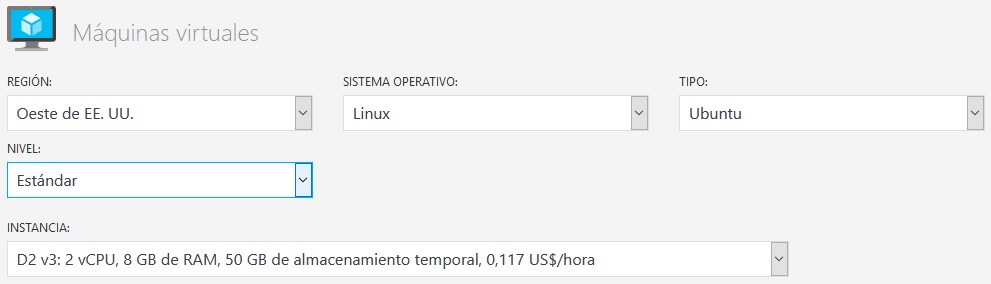
\includegraphics[width=1.0\linewidth]{figure2}}%
%  \subcaptionbox{Another sub-figure\label{fig:rightsubfig}}%
%    {
\includegraphics[width=0.5\linewidth]{knitting-vectorial}}%
  \caption{Precio en Máquinas Virtuales en Azure}
  \label{fig:fig2subfig}
\end{figure}
Para redes virtuales tenemos la \textbf{figura 10.2 Redes Virtuales en Azure}
\begin{figure}[htbp]
 \textbf{Tomado de:} \textit{azure.microsoft.com/en-us/pricing Microsoft Azure}.
  \centering
  %\subcaptionbox{\label{fig:leftsubfig}}%
    {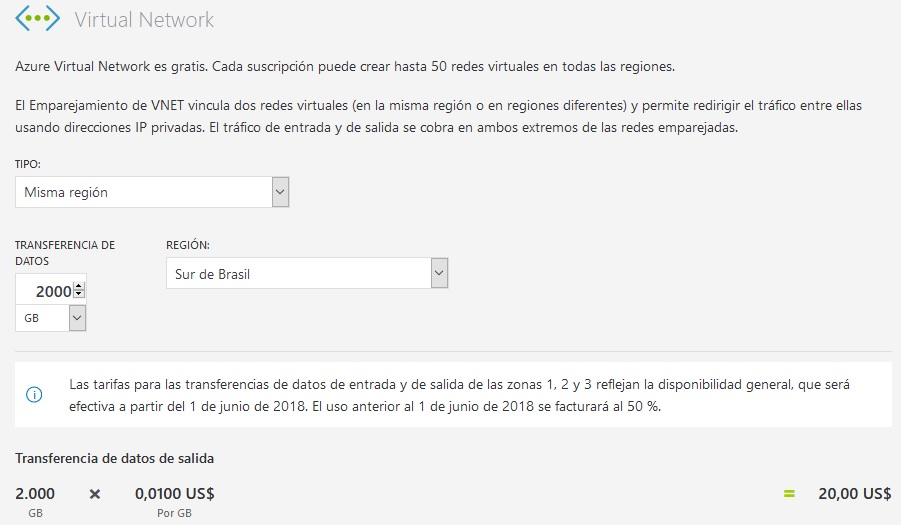
\includegraphics[width=1.0\linewidth]{figure3}}%
%  \subcaptionbox{Another sub-figure\label{fig:rightsubfig}}%
%    {
\includegraphics[width=0.5\linewidth]{knitting-vectorial}}%
  \caption{Precio en Redes Virtuales en Azure}
  \label{fig:fig2subfig}
\end{figure}
%
\\
Podemos encontrar diferentes características, que se requiere en una infraestructura de telecomunicaciones 
Inicie sesión para ver cotizaciones  \textbf{figura 10.3 Infraestructura en Azure}.

*El costo estimado total se basa en los precios aplicables en el día en que se creó la estimación. El costo estimado total real puede variar. Vuelva a abrir el costo estimado para ver el importe total con los precios más recientes
\\
\begin{figure}[htbp]
 \textbf{Tomado de:} \textit{azure.microsoft.com/en-us/pricing Microsoft Azure}.
  \centering
  %\subcaptionbox{\label{fig:leftsubfig}}%
    {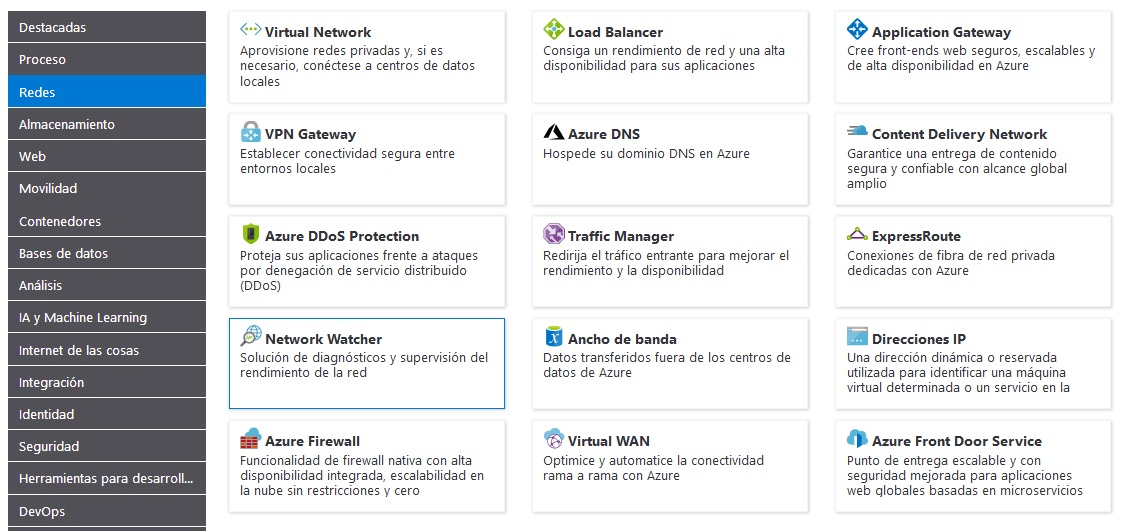
\includegraphics[width=1.0\linewidth]{figure4}}%
%  \subcaptionbox{Another sub-figure\label{fig:rightsubfig}}%
%    {
\includegraphics[width=0.5\linewidth]{knitting-vectorial}}%
  \caption{Diferentes características en Azure para Telecomunicaciones}
  \label{fig:fig2subfig}
\end{figure}

\subsection{Google Cloud}

\textcolor{blue}{Google Cloud:} es una plataforma que ha asociado todas las aplicaciones de desarrollo web que Google 
estaba ofreciendo por separado.
\\
Al adjuntar más servicios en un solo contenedor se desarrolla un fácil administración de los diferentes elementos como almacenamiento, redes, entre otros.

Con Google Cloud se implemento distintos Router para el área diseño de la presente tésis. Los Router que se pudo llegar a implementar fue de la propiedad Cisco el Router CSR 1000v.
\\
Para Google Cloud se puede realizar una estimación de precios en diferentes áreas del mundo ejemplo observamos la \textbf{figura 10.4 Plataform Pricing Calculator}.

\begin{figure}[htbp]
 \textbf{Tomado de:} \textit{cloud.google.com/products Google Cloud}.
  \centering
  %\subcaptionbox{Producto \label{fig:leftsubfig}}%
  %  {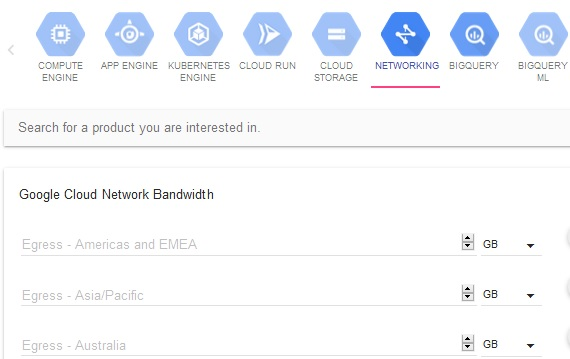
\includegraphics[width=0.4\linewidth]{figure5}}%
 % \subcaptionbox{Estimación\label{fig:rightsubfig}}%
  {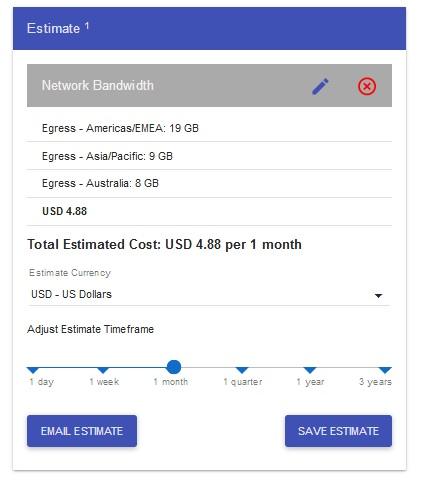
\includegraphics[width=0.8\linewidth]{figure6}}%
  \caption{Plataform Pricing Calculator Google}
  \label{fig:fig2subfig}
\end{figure}

\subsection{Oracle Cloud}

\textcolor{blue}{Oracle:} uno de los más grandes en Base de Datos que enfreta una competencia con IBM desde hace algunos años tiene en sus filas la implementación de Cloud fortaleciendo con grandes herramientas de sistemas opertativos como Linux, también presenta una infratestructura robusta, para instanciar las diferentes máquinas virtuales para nuestro diseño. En la siguiente \textbf{tabla 10.4 Precios Oracle} se detalla la implementación de un Computador con caracteríticas para una empresa entre 100 a 200 empleados.

\begin{table}[ht]
	\caption{Dedicated Compute Classic.}
	\label{tab:hla:results}
\centering
\begin{tabular}{lccccc}
	\toprule
	\multicolumn{1}{c}{\textbf{Product}} 	& \textbf{Price} & \textbf{Metric}\\
	\midrule
\cite{Compute Classic - Model 500} 		& USD \$50,000.00 & 500 OCPUs Month\\
\cite{Compute Classic - Model 1000} 		& USD \$81,000.00 & 1000 OCPUs Month\\
\cite{Compute Classic - Model 1500} 		& USD \$114,000.00 & 1500 OCPUs Month\\
\cite{Compute Classic - Model 2000} 		& USD \$148,000.00 & 2000 OCPUs Month\\

	\midrule
%	\textbf{Total}			& \textbf{--}	\\
	\bottomrule
\end{tabular}
\end{table}

\section{Análisis de Inversión para Cloud} % (fold)
\label{sec:Análisis de Inversión para Cloud}

\subsection{Enfoque al Cliente: Costo, Confiabilidad, Seguridad}
\label{sec:Enfoque al cliente: costo, confiabilidad, seguridad}

Un resumen de investigación de SDxCentral, SD-WAN seguro se ubica entre las tres principales en cuanto a capacidades clave de una red.
El objetivo principal de SD-WAN La tecnología WAN consiste en ofrecer una conexión WAN en la nube, segura y simple, de clase empresarial, con la mayor cantidad de tecnología abierta y basada en software.
Esto se puede usarse para brindar conectividad WAN básica, opara servicios empresariales de primera calidad como VPN, optimización de WAN y control de entrega de aplicaciones (ADC).
\\
\\
Muchas nuevas empresas buscan el potencial en el mercado de WAN definido por software, y las empresas establecidas también están persiguiendo el mercado. Según el IDC, el mercado SD-WAN crecerá a una tasa de crecimiento anual compuesta de 40.4 \% de 2017 a 2022 para llegar a \$ 4.5 mil millones”.
\\
\\
Gartner identifica a los jugadores clave en la tecnología SD-WAN en su Cuadrante Mágico de 2018 para el Informe de Infraestructura de Borde WAN. Nombró a tres líderes: Silver Peak, Cisco y VMware. La firma también reconoció que Riverbed, Citrix, Fortinet, Aryaka y Huawei también son fuertes competidores en el mercado.
\\
\\
Muchos de estos proveedores tienen enfoques del mercado ligeramente diferentes. Por ejemplo, Silver Peak se enfoca en acelerar las aplicaciones de "Software-as-a-Service" (SaaS) en la nube. VMware integró el producto VeloCloud en su propia línea de productos, el VMware NSX SD-WAN de VeloCloud, después de que adquirió VeloCloud
en diciembre de 2017.
\\
\\
El producto contiene aplicaciones de vanguardia, orquestación y puertas de enlace residentes en la nube. Aryaka construyó una red global para que las empresas puedan usar WAN como una red como servicio (NaaS) en cualquier lugar, incluso fuera del área de uno de los puntos de presencia (POP) de Aryaka.
\\
\\
Los proveedores incumbentes de tecnología WAN, como Cisco y Riverbed, que fabrican dispositivos especializados para la conectividad WAN, ahora se centran más en la optimización de WAN y en las ofertas WAN de vanguardia.
Espere que la tendencia se acelere en los próximos años. Lo que comenzó como una
solución para conectividad WAN de sucursales y centros de datos que requieren menos equipos patentados parece expandirse a una amplia gama de ofertas y tecnologías SD-WAN (SDWAN) que incluyen VPN, seguridad, ventaja, optimización de WAN, NaaS y Control de políticas de aplicación.
\\
\\
Si está considerando si SD-WAN mejorará la red de área amplia de su empresa, se ha aprendido que es importante conocer primero las diferentes arquitecturas de SD-WAN.
Como un proveedor de servicios de Internet (ISP) y profesional en este campo  de la nube desde hace
mucho tiempo, he tenido el mejor asiento en la casa para ver cómo la locura de SD-WAN toma vuelo. A medida que aparecen docenas de ofertas de productos SD-WAN, tengo el envidiable trabajo de darle sentido a todo.
\section{Controladores de Negocio SD-WAN}
\label{cha:Controladores de Negocio SD-WAN}


\section{Introducción a SD-WAN}
\label{sec:Introducción a SD-WAN}

Los clientes empresariales exigen tecnologías WAN más flexibles, abiertas y basadas en la nube, en lugar de instalar tecnología WAN patentada o especializada que a menudo involucra costosos circuitos fijos o hardware propietario. Muchas de las nuevas ofertas de WAN definidas por software, por ejemplo, se pueden usar para mejorar y asegurar la conectividad a internet, lo que la hace más competitiva
con tecnologías WAN heredadas más caras como T-1 o MPLS.
\\
\\
Sin embargo, según un estudio de Nemertes, . el 78 \% de las organizaciones que implementan SD-WAN no tienen planes de eliminar completamente el MPLS de su WAN”. En algunos casos, la tecnología WAN definida por software utiliza conexiones de banda ancha de Internet para reemplazar soluciones más caras. La tecnología de virtualización puede aplicar la seguridad y la tecnología de red privada virtual (VPN) a las conexiones
de Internet de banda ancha, lo que las hace más seguras.
\\
\\
Una tendencia notable en el ámbito de las redes es la creciente adopción de la multi-nube en las redes empresariales. La multi-nube es una mezcla de nubes privadas y públicas. Las combinaciones comunes son varias nubes públicas o una nube pública y una nube privada, y cada nube sirve una aplicación empresarial específica.
\textbf{Ver figura 10.5 WAN definida por software (SD-WAN)}.


\begin{figure}[htbp]
 \textbf{Tomado de:} \textit{cisco.com SD-WAN Design}.
  \centering
  %\subcaptionbox{\label{fig:leftsubfig}}%
    {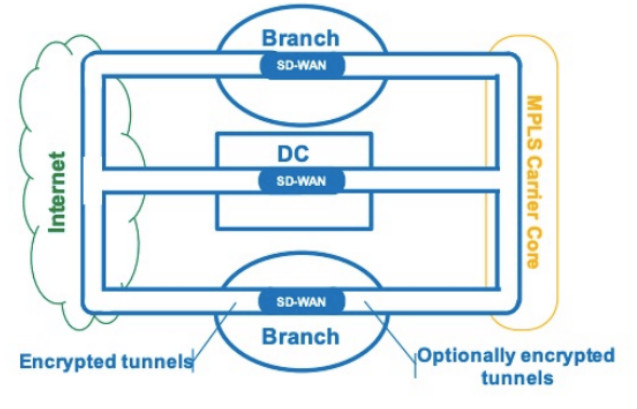
\includegraphics[width=0.8\linewidth]{figure29}}%
%  \subcaptionbox{Another sub-figure\label{fig:rightsubfig}}%
%    {
\includegraphics[width=0.5\linewidth]{knitting-vectorial}}%
  \caption{WAN definida por software (SD-WAN)}
  \label{fig:fig2subfig}
\end{figure}

SD-WAN a menudo se integra en una estrategia de nube múltiple ya que mejora la conectividad y aumenta la seguridad en la nube múltiple. Su escalabilidad en numerosas ubicaciones y su administración centralizada para la nube pública y privada facilitan la administración de la nube múltiple. Varios productos SD-WAN cifran los datos en los puntos de conectividad y proporcionan firewalls y seguridad basada en aplicaciones.
\textbf{Ver figura 10.6 Arquitectura de una SD-WAN}.

\begin{figure}[htbp]
 \textbf{Tomado de:} \textit{cisco.com SD-WAN Design}.
  \centering
  %\subcaptionbox{\label{fig:leftsubfig}}%
    {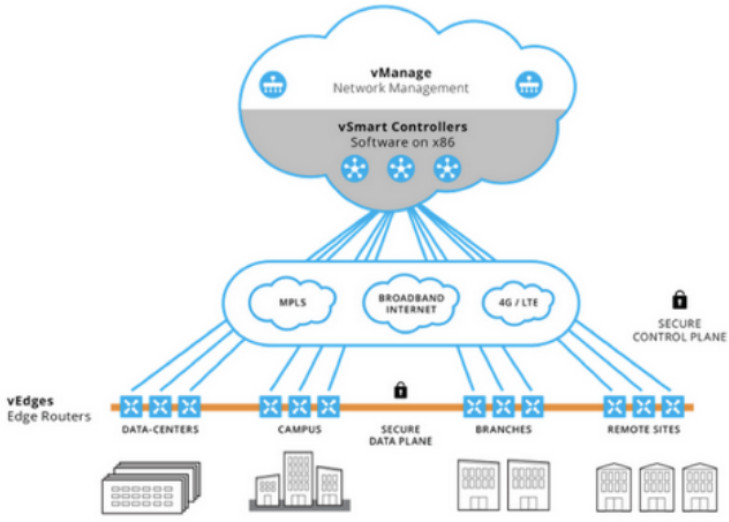
\includegraphics[width=0.8\linewidth]{figure30}}%
%  \subcaptionbox{Another sub-figure\label{fig:rightsubfig}}%
%    {
\includegraphics[width=0.5\linewidth]{knitting-vectorial}}%
  \caption{Arquitectura de una SD-WAN}
  \label{fig:fig2subfig}
\end{figure}


\section{Tipos de Arquitectura SD-WAN}
\label{sec:Tipos de Arquitectura SD-WAN}

\subsection{Enfoque de una SD-WAN}
\label{sec:Enfoque de una SD-WAN}

Una arquitectura SD-WAN (esencialmente es un enrutador "plug-and-play"), que realiza
la configuración del tráfico en tiempo real en cada sitio. A diferencia de otras arquitecturas, el cuadro SD-WAN en el sitio no se conecta a una puerta de enlace en la nube, solo se conecta a los otros sitios de su empresa.

\subsubsection{Mejor Ajuste}
\label{sec:Mejor Ajuste}

Empresas que alojan todas sus aplicaciones en la empresa (sin ninguna aplicación en la nube), su empresa no utiliza aplicaciones en la nube, no es necesario utilizar una solución SD-WAN habilitada para la nube. Agregar la habilitación de la nube aumentará los costos, innecesariamente. Una configuración común es mantener una red MPLS (mucho más pequeña) para aplicaciones en tiempo real (es decir, voz, video o escritorio virtual), y utilizar la Internet pública (controlada por SD-WAN) para todo lo demás.

\subsubsection{Beneficios}
\label{sec:Beneficios}

Equilibrio de carga multi-circuito / ISP. Conformación del tráfico en tiempo real, que mejora el rendimiento de todas las aplicaciones WAN. Mejor recuperación de desastres (DR), al tener una mejor copia de seguridad de conectividad.

\subsection{Cloud}
\label{sec:Cloud}


En una arquitectura SD-WAN habilitada para la nube, la solución de una SD-WAN en el sitio que se conecta a una puerta de enlace (virtual) en la nube. Con esta arquitectura, su empresa obtiene los beneficios de una arquitectura (es decir, configuración de tráfico en tiempo real y balanceo de carga de múltiples circuitos), además de un mayor rendimiento y confiabilidad de sus aplicaciones en la nube.
\\
\\
La puerta de enlace de la nube está conectada en red directamente a los principales proveedores de la nube (es decir, Office 365, AWS, Salesforce, etc.), lo que se traduce un mejor rendimiento de sus aplicaciones en la nube. Además, si el circuito de Internet de su empresa falla al usar una aplicación en la nube, la puerta de enlace puede mantener una sesión en la nube activa (mientras que el circuito falla). Si su empresa tiene un circuito de Internet alternativo, la SD-WAN puede redirigir su aplicación en la nube de forma instantánea al circuito de Internet alternativo de su empresa, evitando la interrupción de una sola sesión


\subsubsection{Mejor Ajuste}
\label{sec:Mejor Ajuste}

Compañías que ejecutan aplicaciones en la nube de renombre, como Office 365, AWS, Drop Box, Azure, Salesforce, etc. Una configuración común es tener aplicaciones internas en tiempo real que se ejecutan en una pequeña red MPLS y tener aplicaciones en la nube, corriendo sobre la Internet pública, controlada por una SD-WAN.

\subsubsection{Beneficios}
\label{sec:Beneficios}

\begin{itemize}
\item[•] \textbf{Cloud gateways, mejorando el rendimiento de las aplicaciones en la nube.}
\item[•] \textbf{Cloud gateways, mejorando la fiabilidad de las aplicaciones en la nube.}
\item[•] \textbf{Equilibrio de carga multi-circuito / ISP.}
\item[•] \textbf{Conformación del tráfico en tiempo real, que mejora el rendimiento de todas las aplicaciones WAN.}
\item[•] \textbf{DR mejorado por tener una mejor copia de seguridad de conectividad.}
\end{itemize}

\subsection{Cloud Backbone}
\label{sec:Cloud Backbone}

Siempre es bueno tener una columna vertebral, ¿verdad? La arquitectura SD-WAN habilitada para la nube se puede llevar a otro nivel cuando obtiene una red troncal. La arquitectura SD-WAN habilitada para la nube más la red troncal que conecta su sitio con el punto de presencia de red (POP) más cercano del proveedor de SD-WAN, donde su tráfico salta en la parte privada del proveedor de SD-WAN. Fibra óptica, red troncal.
\\
\\
Mientras el tráfico de su WAN atraviesa la red troncal privada del proveedor de SD-WAN, se garantiza que mantendrá bajos niveles de latencia, pérdida de paquetes y fluctuaciones.
Esto mejora el rendimiento de todo el tráfico de red, particularmente el tráfico en tiempo real como voz, video y escritorio virtual. La red troncal también está conectada directamente con los principales proveedores de aplicaciones en la nube (es decir, Office 365, AWS, etc.), que, al igual que la arquitectura anterior, aumenta el rendimiento y la confiabilidad de esas aplicaciones.

\subsubsection{Mejor Ajuste}
\label{sec:Mejor Ajuste}
Una empresa que ejecuta una gran cantidad de aplicaciones de red en tiempo real, que desea eliminar completamente su red MPLS (para reducir los costos), pero no quiere que su tráfico en tiempo real se desplace al 100 \% a través de la Internet pública (por temor a una alta latencia, paquetes pérdida y jitter).

\subsubsection{Beneficios}
\label{sec:Beneficios}

El tráfico de WAN se basa principalmente en una red troncal privada, lo que mejora el rendimiento de todas las aplicaciones de red, especialmente las aplicaciones en tiempo real.

Actualmente no hay muchos proveedores que ofrezcan esta arquitectura. Sin embargo, como muchos ISP han agregado el servicio SD-WAN a su cartera de productos (ya que los ISP ya tienen la infraestructura de red troncal), solo tiene sentido que varios ISP finalmente agreguen esta opción a su oferta de SD-WAN. Suena bastante simple, ¿verdad? Así un poco. Por supuesto, dentro de cada una de estas 3 arquitecturas hay varias variables más, pero creo que esto le brinda un comienzo sólido para evaluar y diseñar con precisión una solución SD-WAN para su empresa.


\section{Selección de Proveedor y Tecnología} % (fold)
\label{sec:Selección de Proveedor y Tecnología}

Para la selección de la solución específica que se diseña tenemos en cuenta los costos de cada una de ella y por supuesto las ventajas en términos de servicio que obtendría el cliente, el principal criterio de selección es utilizar la solución que cumpla con los objetivos del proyecto sin implicar costos demasiado grandes para el cliente. Teniendo esto en cuenta debemos considerar la solución actual del cliente.
\\
\\
Hace poco tiempo el cliente migró su infraestructura de unos equipos Mikrotik a dispositivos Cisco, por lo que de ser posible el proyecto debe conservar dichos equipos para no perder la inversión realizada por el cliente. La migración realizada fue de equipos Mikrotik a equipos Cisco 891 en las diferentes tiendas y equipos Cisco 4331 en las regionales y la sede nacional.
\\
\\
Dados los criterios definidos anteriormente se procede a analizar cada una de las soluciones que se plantearon para el desarrollo del proyecto.
\\
\\
La primera opción que se consideró fue utilizar OpenDayLight como controlador SD-WAN ya que este utiliza totalmente software abierto para su funcionamiento, esta plataforma utiliza protocolos abiertos como  Openflow y Netconf, \textbf{Ver figura 10.7 Solución de la Arquitectura}.



\begin{figure}[htbp]
 \textbf{Tomado de:} \textit{OpenDayLight.org Solución de la Arquitectura OpenDayLight}.
  \centering
  %\subcaptionbox{\label{fig:leftsubfig}}%
    {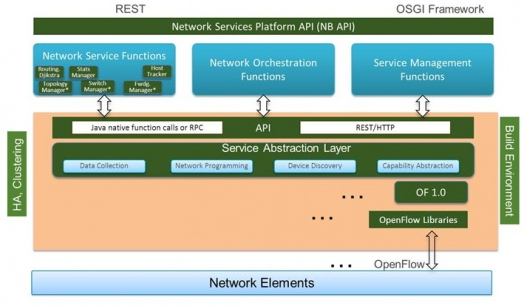
\includegraphics[width=0.9\linewidth]{figure31}}%
%  \subcaptionbox{Another sub-figure\label{fig:rightsubfig}}%
%    {
\includegraphics[width=0.5\linewidth]{knitting-vectorial}}%
  \caption{Solución de la Arquitectura}
  \label{fig:fig2subfig}
\end{figure}

Esta arquitectura aunque al utilizar protocolos estándar permite que se conecte cualquier elemento de red que hable Openflow tiene la limitante de que los equipos de red tradicionales, incluyendo los que tiene el cliente no soportan OpenFlow por defecto, y por tanto los enrutadores que utiliza el cliente hoy en día no se integran con esta arquitectura de SDN, lo que significa que implementar esta solución requeriría cambiar todos los enrutadores por unos que soporten OpenFlow.
\\
\\
Se tuvieron en cuenta también soluciones de varios fabricantes para el proyecto, más precisamente las soluciones SD-WAN de Nokia(Nuage), Cisco(Viptela), vmware(Velo cloud) y Silverpeak, estas son las soluciones que dominan el mercado a la fecha de elaboración de este documento. Todas estas son soluciones SDN \textbf{Ver figura 10.8 Solución y Funcionamiento de una red SD-WAN}. que desagregan completamente los planos de control y gestión de los enrutadores en las sedes Branch y los centralizan en controladoras y servidores de gestión, aunque todas las soluciones mencionadas utilizan protocolos diferentes su arquitectura y funcionamiento es muy similar.
\begin{figure}[htbp]
 \textbf{Tomado de:} \textit{cisco.com Solución y Funcionamiento de una red SD-WAN}.
  \centering
  %\subcaptionbox{\label{fig:leftsubfig}}%
    {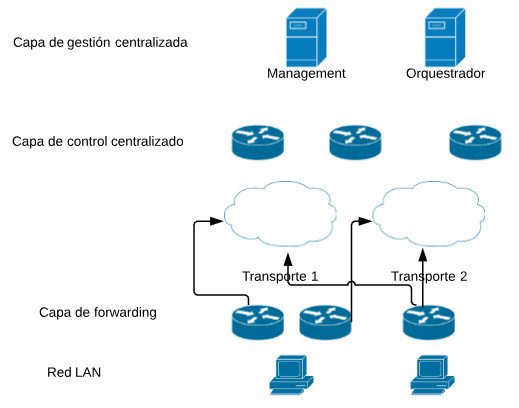
\includegraphics[width=0.9\linewidth]{figure32}}%
%  \subcaptionbox{Another sub-figure\label{fig:rightsubfig}}%
%    {
\includegraphics[width=0.5\linewidth]{knitting-vectorial}}%
  \caption{Solución y Funcionamiento de una red SD-WAN}
  \label{fig:fig2subfig}
\end{figure}
Dentro de cada una de estas opciones se desagregan las capas de control y de gestión en un sitio centralizado, normalmente un centro de datos, y en los branch solamente se tiene la capa de envío de datos o forwarding, estas sedes remotas se comunican entre ellas en todos los casos mediante túneles que se forman automáticamente gracias al plano de control centralizado, sin embargo la tecnología con la que se forman dichos túneles y con la que se envía la información de enrutamiento del plano de control al plano de forwarding cambia considerablemente entre todas las soluciones, y por tanto son incompatibles entre ellos. Las siguientes son las tecnologías que cada una de las soluciones mencionadas utiliza para la comunicación contra los routers de borde:
\begin{itemize}
\item[•]\textbf{Nokia (nuage): Openflow}
\item[•]\textbf{Cisco (Viptela): Netconf, OMP}
\item[•]\textbf{Vmware (VeloCloud):Dynamic multipath Optimization}
\item[•]\textbf{Silverpeak: Dynamic path control}
\end{itemize}
Podemos ver entonces que los enrutadores tradicionales no soportan ninguno de los protocolos de los diferentes fabricantes, por tanto cada fabricante desarrolla sus propios routers de borde para su solución SD-WAN, y por esta razón la implementación de cualquiera de estas soluciones implicaría un reemplazo total de los equipos.
\\
\\
Existe una solución SD-WAN de Cisco basada en los enrutadores tradicionales llamada IWAN, esta solución combina diferentes protocolos ya activos en los enrutadores tradicionales: EIGRP, DMVPN, PfR, WAAS y NBAR para generar una solución basada en aplicaciones que balancee y enrute el tráfico de forma inteligente en la red, todo automatizado a través de su controlador SDN: APIC-EM. Los enrutadores con los que cuenta el cliente soportan cada una de las aplicaciones aquí mencionadas y por tanto esta sería la única solución que no requiere un reemplazo total de los equipos del cliente.
\\
\\
Por esta razón IWAN fue la solución seleccionada para el desarrollo de este proyecto, ya que de otra forma la inversión que se requeriría al reemplazar todos los enrutadores del cliente con cualquiera de las demás soluciones aquí consideradas sería tan alta que impediría el desarrollo del proyecto, ya que el capital con el que se cuenta para el desarrollo del mismo es limitado.

\section{Ventajas y Desventajas de la Solución Propuesta} % (fold)
\label{sec:Ventajas y Desventajas de la Solución Propuesta}

Esta sección permite establecer las ventajas y desventajas del uso de la tecnología SD-WAN seleccionada en comparación con la solución actual que tiene el cliente en sus equipos.
\\
\\
Una de las ventajas más notorias es el tiempo que se ahorra en los procesos tanto de implementación como de cambios, a continuación hay un comparativo de los tiempos para la nueva solución y para la solución anterior \textbf{tabla 10.5 Implementación y Ahorro de Precios en SD-WAN}.

%\begin{table}[ht]
%	\caption{Amazon EC2 Pricing.}
%	\label{tab:hla:results}
%\centering
%\begin{tabular}{lccccc}
%	\toprule
%	\multicolumn{1}{c}{\textbf{Proceso}} 	& \textbf{IWAN}	& \textbf{Tiempo}	& \textbf{Solución Actual}
%	& \textbf{Tiempo}\\
%	\midrule
%\cite{Aprovisionamiento tienda nueva} 		& N/A & 2GiB & EBS Only	& \$0.0255 per Hour \\
%\cite{a1.large}~2 		& N/A & 4GiB & EBS Only & \$0.051 per Hour	\\
%\cite{a1.xlarge}~4		& N/A & 4GiB & EBS Only & \$0.051 per Hour	\\
%\cite{a1.2xlarge}~8 	& N/A & 16GiB & EBS Only & \$0.204 per Hour	\\
%\cite{a1.4xlarge}~16	& N/A & 32GiB & EBS Only & \$0.408 per Hour	\\
%\cite{t3.nano}~2		& N/A & 0.5GiB & EBS Only & \$0.0052 per Hour	\\
%\cite{t3.micro}~2   	& N/A & 1GiB & EBS Only & \$0.0104 per Hour	\\
%	\midrule
%	\textbf{Total}			& \textbf{--}		& \textbf{--}		& \textbf{--} \\
%	\bottomrule
%\end{tabular}
%\end{table}
\begin{table}[ht]
\caption{Implementación y Ahorro de Precios en SD-WAN}
\label{tabla:autores}
\centering
\begin{tabular}{p{3.5cm} p{2.5cm} p{1.5cm} p{5cm} p{1.5cm}}
\hline
\textbf{Proceso} & \textbf{IWAN} & \textbf{Tiempo} & \textbf{Solución Actual} & \textbf{Tiempo}\\
\hline
\textbf{Aprovisionamiento tienda nueva} & Se ingresan datos básicos sobre el APIC-EM  & 30min & 
Se configura túnel en la tienda y en la regional y enrutamiento hacia internet y hacia las tiendas. & 3h \\
\hline
\textbf{Aprovisionamiento regional nueva} & Se ingresan datos básicos sobre el APIC-EM & 30min & 
Se deben configurar túneles IPSEC contra todas las demás regionales, además de configurar protocolos de enrutamiento dinámico contra el proveedor y contra las demás regionales por medio del canal de internet. & 2d \\
\hline
\textbf{Cambio general de políticas} & Se configura script y se agenda para ser aplicado en todos los equipos & 1h & 
Se ingresa equipo por equipo a realizar los cambios manualmente. & 4meses \\
\hline
\end{tabular}
\end{table}

Adicional a los tiempos, las dos soluciones tienen diferencias importantes a nivel de servicio por lo que la siguiente tabla muestra en detalle dichas diferencias para establecer qué solución conviene más para las necesidades del negocio \textbf{tabla 10.6 Necesidades de Negocio SD-WAN}.

\begin{table}[ht]
\caption{Necesidades de Negocio SD-WAN}
\label{tabla:autores}
\centering
\begin{tabular}{p{3.5cm} p{5.5cm} p{5.5cm} }
\hline
\textbf{Caractéristica} & \textbf{IWAN} & \textbf{Solución Legacy} \\
\hline
\textbf{Redundancia} & 4 puntos concentradores de la solución, principal y backup de intranet y principal y backup de internet.  & único punto de falla, si el internet de la regional cae, cae la conexión de todas las tiendas asociadas a dicha regional.\\
\hline
\textbf{Calidad de Servicio} & Por aplicación, utilizando NBAR para la identificación y priorización de aplicaciones. & Por redes o por puerto, la clasificación se realiza en capa 4 del modelo OSI. \\
\hline
\textbf{Balanceo de Carga} & Nativo, se utiliza PfR para validar según las necesidades de la aplicación, cuál es el mejor camino para enviar el tráfico. & Es posible el balanceo pero este sería estático, si algún enlace está degradado igualmente se enviará tráfico a través de él. \\
\hline
\end{tabular}
\end{table}

Como puede verse en ambas tablas, la solución de IWAN genera ventajas tanto en tiempos como en costos y en redundancia y servicio, por lo que en general está más alineada con las necesidades del negocio.

\section{Requerimientos de Aplicaciones} % (fold)
\label{sec:Requerimientos de Aplicaciones}

Este diseño se encuentra enfocado a las aplicaciones del cliente, por lo que este capítulo está enfocado a determinar los requerimientos de ancho de banda, latencia y jitter para las aplicaciones críticas del cliente, esto con el fin de establecer un diseño de QoS y para definir el ancho de banda necesario en los enlaces, cabe aclarar que el uso de estas aplicaciones cambia en los 3 tipos de sedes definidos en el proyecto. Las aplicaciones definidas por el cliente son las siguientes:
\begin{itemize}
\item[•]\textbf{Telefonía:} telefonía IP en todas las sedes, un telefóno IP por tienda y un segmento de red para telefonía en cada una de las regionales y en la sede nacional, este servicio de telefonía utiliza SIP como protocolo de señalización y túneles IAX entre las plantas telefónicas, hay una planta telefónica en cada regional a donde se registran los teléfonos de cada tienda, a continuación se muestra el diagrama general del servicio de telefonía actualmente. \textbf{Ver figura 10.9 Telefonía}.
\begin{figure}[htbp]
 \textbf{Tomado de:} \textit{cisco.com Cisco SD-WAN Design Guide}.
  \centering
  %\subcaptionbox{\label{fig:leftsubfig}}%
    {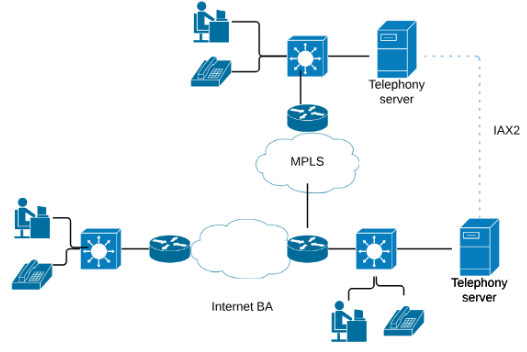
\includegraphics[width=0.9\linewidth]{figure33}}%
%  \subcaptionbox{Another sub-figure\label{fig:rightsubfig}}%
%    {
\includegraphics[width=0.5\linewidth]{knitting-vectorial}}%
  \caption{Telefonía}
  \label{fig:fig2subfig}
\end{figure}

\item[•]\textbf{FTP:}Cada una de las tiendas realiza un proceso de inventariado semanalmente, estos archivos de inventario son subidos a un servidor FTP en la sede nacional de Medellín, por lo tanto el servicio de FTP es considerado como crítico para el negocio.
\item[•]\textbf{Videoconferencia:} el cliente utiliza un servicio de videoconferencia en la nube, más específicamente google Hangouts, que para una calidad óptima de video utiliza 3.2Mbps por videoconferencia, por lo que es una de las aplicaciones que más consumo de ancho de banda genera, es además una de las aplicaciones más críticas para la compañía, ya que es utilizada por los altos directivos.
\item[•]\textbf{CCTV:} el cliente monitorea mediante el enlace de internet de las tiendas, todas la plataforma de CCTV, por lo que se debe garantizar el acceso desde internet a esta aplicación.
\item[•]\textbf{Servicios Web privados:} el cliente cuenta con una Intranet en la que las tiendas y las regionales realizan procesos corporativos vitales para la empresa, de igual forma al hacer parte de un grupo empresarial, consumen en forma de servicios Web aplicaciones en datacenter de otros miembros del grupo empresarial.
\item[•]\textbf{Internet:} desde cada una de las tiendas y las regionales se tiene acceso a internet para navegación, sin embargo este no es un servicio crítico para el cliente.

\item[•]\textbf{Escritorio Remoto:} el grupo de soporte de TI requiere conectividad por escritorio remoto a regionales y tiendas de manera que se pueda realizar un soporte remoto de aplicaciones y equipos de computo.

\item[•]\textbf{Correo:} el cliente cuenta con buzones de correo de google que acceden mediante sus enlaces a internet.
\end{itemize}
Los requerimientos de ancho de banda, jitter y delay así como la criticidad de cada servicio se resumen en la siguiente \textbf{tabla 10.7 Características de Calidad de Servicio en un SD-WAN}:

\begin{table}[ht]
	\caption{Características de Calidad de Servicio en un SD-WAN}
	\label{tab:hla:results}
\centering
\begin{tabular}{lccccc}
	\toprule
	\multicolumn{1}{c}{\textbf{Aplicación}} 	& \textbf{BW}	& \textbf{Delay}	& \textbf{Jitter} 	& \textbf{Packet Loss} & \textbf{Description}\\
	\midrule
\cite{Telefonia} 		& 80kbps call & 150ms max & 30ms max	& 1\% max & Mission-critical\\
\cite{Videoconferencia} & 3.2Mbps & 150ms max & 30ms max & 1\% max & Mission-critical\\
\cite{FTP} 		& 3Mbps & tolerant & tolerant& 5\% max & Mission-critical\\
\cite{CCTV} 		& 2Mbps & 1s max & tolerant	& 2\% max & Business-class\\
\cite{Web Privada} 		& 1Mbps & tolerant & tolerant & 5\% max & Business-class\\
\cite{Internet} 		& 1Mbps & tolerant & tolerant & 5\% max & Best effort\\
\cite{Escritorio remoto} & 2Mbps & 200ms max & 30ms max	& 1\% max & Business-class\\
\cite{Correo} & 1Mbps & tolerant & tolerant	& 5\% max & Best effort\\
	\midrule
	\textbf{Total}			& \textbf{--}		& \textbf{--}		& \textbf{--} \\
	\bottomrule
\end{tabular}
\end{table}

\section{Requerimientos de Ancho de Banda} % (fold)
\label{sec:Requerimientos de Ancho de Banda}

Con cada una de las aplicaciones descritas se procede a calcular por tanto el ancho de banda requerido en cada una de las sedes, y se genera una estadística del consumo actual en cada una de esas sedes para establecer tanto de manera teórica como práctica el ancho de banda requerido en cada uno de los tipos de sedes remotas y en el centro de datos. \textbf{Algoritmo para Diseño de SD-WAN Anexo III}
\\
\\
Se realiza un análisis del consumo actual de ancho de banda del cliente utilizando las herramientas de monitoreo disponibles y se obtienen los siguientes datos de consumo para cada una de las 11 sedes regionales y nacionales \textbf{tabla 10.8 Análisis de consumo en las Sedes}:
\begin{table}[ht]
	\caption{Análisis de consumo en las Sedes}
	\label{tab:hla:results}
\centering
\begin{tabular}{lccccc}
	\toprule
	\multicolumn{1}{c}{\textbf{Sede}} 	& \textbf{Consumo Promedio}	& \textbf{BW Contratado}\\
	\midrule
\cite{Nacional Medellin} 		& 14Mbps & 14Mbps \\
\cite{Antioquia Norte} 		& 20Mbps & 15Mbps \\
\cite{Nacional Tocancipa} 		& 20Mbps & 20Mbps \\
\cite{Soacha} 		& 7Mbps & 7Mbps \\
\cite{Antioquia Sur} 		& 7Mbps & 7Mbps \\
\cite{Antioquia Oriente} 		& 7Mbps & 7Mbps \\
\cite{Eje Cafetero} 		& 14Mbps & 7Mbps \\
\cite{Valle} 		& 13Mbps & 7Mbps \\
\cite{Cota} 		& 7Mbps & 7Mbps \\
\cite{Bucaramanga} 		& 7Mbps & 7Mbps \\
\cite{Funza} 		& 8Mbps & 7Mbps \\
	\midrule
	\textbf{Total}			& \textbf{--}		& \textbf{--} \\
	\bottomrule
\end{tabular}
\end{table}

Con estos datos se puede concluir que ya hay saturación en las sedes, y que por tanto la solución actual está presentando retardos y pérdidas de paquetes en la comunicación.
Se toman muestras de tráfico utilizando el protocolo Netflow con el fin de caracterizar el tráfico de cada una de las aplicaciones obteniendo los siguientes resultados:

\subsection{Sede Nacional Tocancipá:} % (fold)
\label{sec:Sede Nacional Tocancipá:}

\textbf{Ver figura 10.10 Sede Nacional Tocancipá}.
\begin{figure}[htbp]
  \centering
  %\subcaptionbox{\label{fig:leftsubfig}}%
    {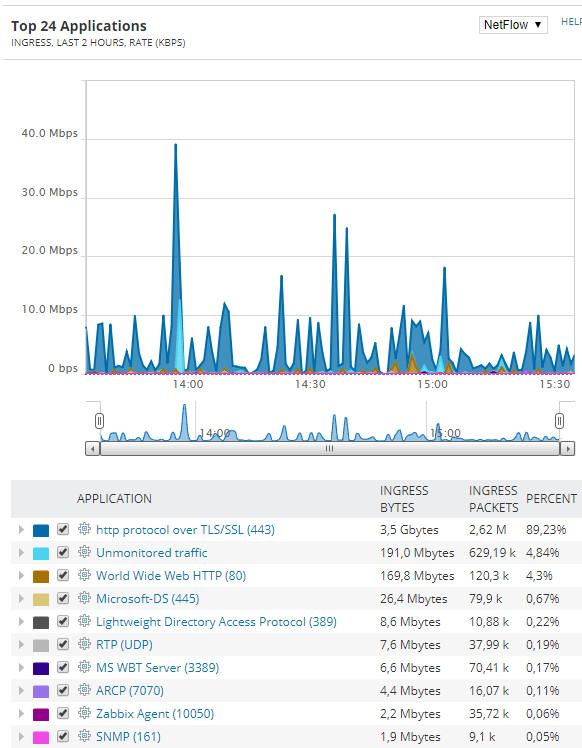
\includegraphics[width=1.0\linewidth]{figure34}}%
%  \subcaptionbox{Another sub-figure\label{fig:rightsubfig}}%
%    {
\includegraphics[width=0.5\linewidth]{knitting-vectorial}}%
  \caption{Sede Nacional Tocancipá}
   \textbf{Tomado de:} \textit{autores}.
  \label{fig:fig2subfig}
\end{figure}

\subsection{Sede Nacional Medellín:} % (fold)
\label{sec:Sede Nacional Medellín:}

\textbf{Ver figura 10.11 Sede Nacional Medellín}.
\begin{figure}[htbp]
  \centering
  %\subcaptionbox{\label{fig:leftsubfig}}%
    {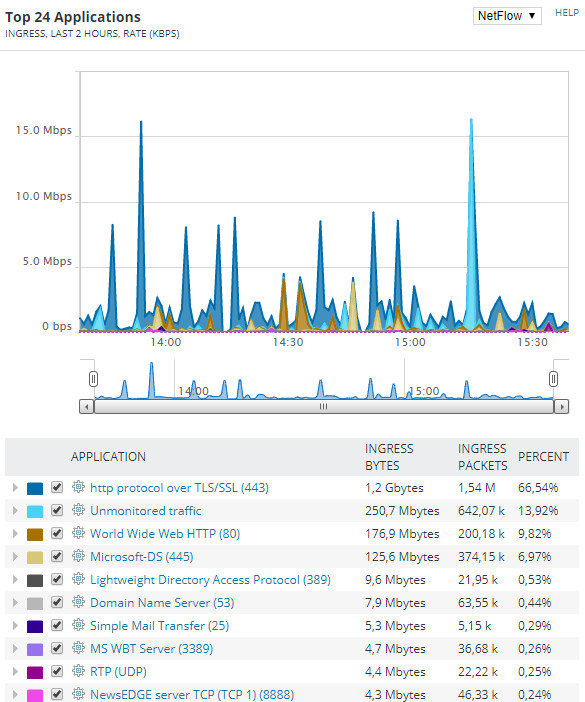
\includegraphics[width=1.0\linewidth]{figure35}}%
%  \subcaptionbox{Another sub-figure\label{fig:rightsubfig}}%
%    {
\includegraphics[width=0.5\linewidth]{knitting-vectorial}}%
  \caption{Sede Nacional Medellín}
   \textbf{Tomado de:} \textit{autores}.
  \label{fig:fig2subfig}
\end{figure}

\subsection{Sede Nacional Antioquia Norte:} % (fold)
\label{sec:Sede Nacional Antioquia Norte:}

\textbf{Ver figura 10.12 Sede Nacional Antioquia Norte}.
\begin{figure}[htbp]
  \centering
  %\subcaptionbox{\label{fig:leftsubfig}}%
    {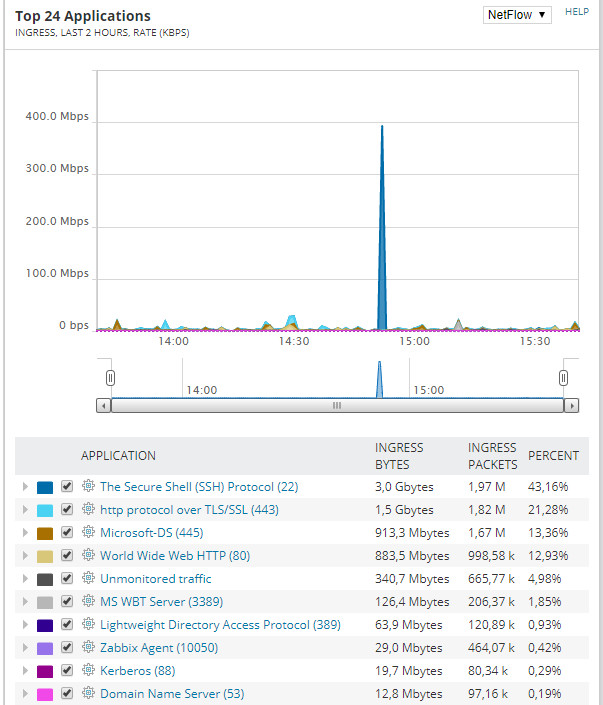
\includegraphics[width=1.0\linewidth]{figure36}}%
%  \subcaptionbox{Another sub-figure\label{fig:rightsubfig}}%
%    {
\includegraphics[width=0.5\linewidth]{knitting-vectorial}}%
  \caption{Sede Nacional Antioquia Norte}
   \textbf{Tomado de:} \textit{autores}.
  \label{fig:fig2subfig}
\end{figure}

\subsection{Sede Nacional Antioquia Norte:} % (fold)
\label{sec:Sede Nacional Antioquia Norte:}

\textbf{Ver figura 10.13 Sede Nacional Valle}.
\begin{figure}[htbp]
  \centering
  %\subcaptionbox{\label{fig:leftsubfig}}%
    {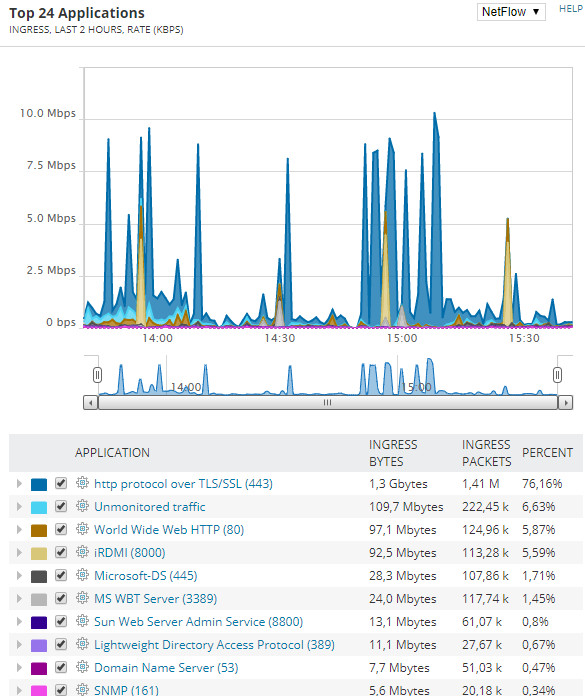
\includegraphics[width=1.0\linewidth]{figure37}}%
%  \subcaptionbox{Another sub-figure\label{fig:rightsubfig}}%
%    {
\includegraphics[width=0.5\linewidth]{knitting-vectorial}}%
  \caption{Sede Nacional Valle}
   \textbf{Tomado de:} \textit{autores}.
  \label{fig:fig2subfig}
\end{figure}

De estos resultados se concluye que para todos los casos el Tráfico Web representa la gran mayoría del tráfico que se genera tanto en las regionales como en las sedes nacionales
\\
\\
El tráfico en todos los casos se encuentra al límite de la capacidad, las herramientas de monitoreo no muestran pérdidas de paquetes pero si latencias y jitter que puede afectar la calidad del tráfico de voz y las videoconferencias, adicionalmente en la actualidad no habría posibilidad de crecimiento, teniendo en cuenta el nivel de consumo actual se definen los siguientes anchos de banda para el proyecto \textbf{tabla 10.9 Ancho de Banda para los Proyectos}:

\begin{table}[ht]
	\caption{Ancho de Banda para los Proyectos}
	\label{tab:hla:results}
\centering
\begin{tabular}{lccccc}
	\toprule
	\multicolumn{1}{c}{\textbf{Sede}} 	& \textbf{Consumo Promedio}	& \textbf{BW MPLS} & \textbf{BW}\\
	\midrule
\cite{Nacional Medellin} 		& 14Mbps & 15Mbps  & 20Mbps \\
\cite{Antioquia Norte} 		& 20Mbps & 20Mbps & 50Mbps\\
\cite{Nacional Tocancipa} 		& 20Mbps & 20Mbps & 20Mbps \\
\cite{Soacha} 		& 7Mbps & 10Mbps & 20Mbps \\
\cite{Antioquia Sur} 		& 7Mbps & 10Mbps & 20Mbps \\
\cite{Antioquia Oriente} 		& 7Mbps & 10Mbps & 20Mbps \\
\cite{Eje Cafetero} 		& 14Mbps & 15Mbps & 20Mbps \\
\cite{Valle} 		& 13Mbps & 15Mbps & 20Mbps \\
\cite{Cota} 		& 7Mbps & 10Mbps & 20Mbps \\
\cite{Bucaramanga} 		& 7Mbps & 10Mbps & 20Mbps \\
\cite{Funza} 		& 8Mbps & 10Mbps & 20Mbps \\
	\midrule
	\textbf{Total}			& \textbf{--}		& \textbf{--} \\
	\bottomrule
\end{tabular}
\end{table}

\section{Diseño del DataCenter}
\label{sec:Diseño del DataCenter}

El diseño del centro del centro de datos se realiza de acuerdo a las mejores prácticas dadas por Cisco en su guía de diseño, para esta solución la topología utilizada es la que Cisco llama diseño híbrido de IWAN, ya que se requieren dos medios de transporte independientes, MPLS e internet banda ancha. \textbf{Ver figura 10.1 Diseño de DataCenter}.
\begin{figure}[htbp]
  \centering
  %\subcaptionbox{\label{fig:leftsubfig}}%
    {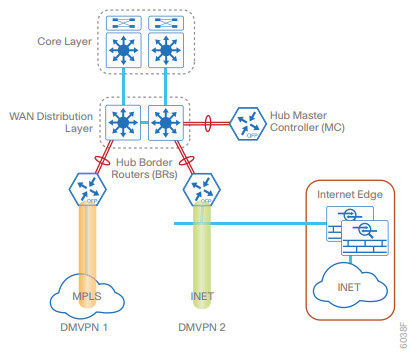
\includegraphics[width=0.6\linewidth]{figure38}}%
%  \subcaptionbox{Another sub-figure\label{fig:rightsubfig}}%
%    {
\includegraphics[width=0.5\linewidth]{knitting-vectorial}}%
  \caption{Diseño de DataCenter}
   \textbf{Tomado de:} \textit{autores}.
  \label{fig:fig2subfig}
\end{figure}

En este diseño se requiere acceso a los dos transportes desde el centro de datos, en el datacenter se encuentran los Hub Border routers que son quienes lo interconectan con las dos tecnologías de transporte y el Master controller, estos equipos estarán conectados mediante una infraestructura de switches(existente) que soporta PIM y otras tecnologías de multicast para el correcto funcionamiento del plano de control.
\\
\\
Se sugiere al cliente por redundancia tener dos centros de datos con esta topología para garantizar la alta disponibilidad de la solución, sin embargo por costos el cliente indica que no es posible contar con una topología de ese estilo, por ende se garantiza disponibilidad de equipos en un solo centro de datos para que la falla de algún equipo de borde no genere afectación en el plano de datos del cliente, la topología adoptada para esta solución es la siguiente \textbf{Ver figura 10.14 Topología de DataCenter}.

\begin{figure}[htbp]
  \centering
  %\subcaptionbox{\label{fig:leftsubfig}}%
    {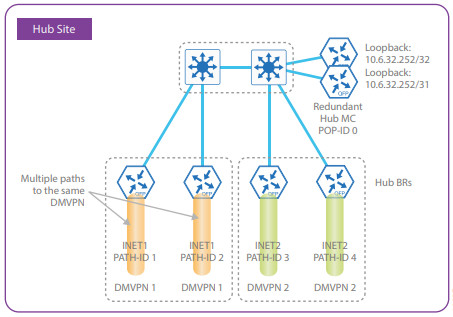
\includegraphics[width=0.6\linewidth]{figure39}}%
%  \subcaptionbox{Another sub-figure\label{fig:rightsubfig}}%
%    {
\includegraphics[width=0.5\linewidth]{knitting-vectorial}}%
  \caption{Topología de DataCenter}
   \textbf{Tomado de:} \textit{autores}.
  \label{fig:fig2subfig}
\end{figure}

De esta manera, para cada tecnología de transporte se tendrán dos Hub Border Router para garantizar la redundancia en la terminación de túneles DMVPN contra el datacenter, de igual forma la redundancia del plano de control se da mediante la utilización de dos Master controller en el centro de datos.
\\
\\
Sin embargo con el fin de disminuir la cantidad de equipos que deben ser adquiridos por el cliente para la implementación de la solución se utiliza la tecnología MTT (Multiple Tunnel Termination), esto permite utilizar únicamente dos HBR(Hub Border Router) en el centro de datos y establecer la redundancia configurando múltiples túneles en cada equipo, la siguiente imagen muestra la idea general de esta tecnología \textbf{Ver figura 10.15 Configuración de Túneles para el DataCenter}.

\begin{figure}[htbp]
  \centering
  %\subcaptionbox{\label{fig:leftsubfig}}%
    {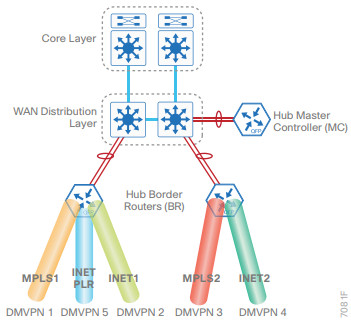
\includegraphics[width=0.6\linewidth]{figure40}}%
%  \subcaptionbox{Another sub-figure\label{fig:rightsubfig}}%
%    {
\includegraphics[width=0.5\linewidth]{knitting-vectorial}}%
  \caption{Configuración de Túneles para el DataCenter}
   \textbf{Tomado de:} \textit{autores}.
  \label{fig:fig2subfig}
\end{figure}

Por lo que al final el diseño utilizaría dos equipos para realizar la función de HBR, cada uno terminando túneles hacia los dos transportes (internet banda ancha y MPLS) y dos equipos para hacer la función de MC.
\\
\\
La función del MC es definir las políticas de PfR que se utilizarán para el balanceo de carga y los requerimientos de cada una de las aplicaciones que componen la solución, para este cliente se definen agruparon las aplicaciones en ciertos grupos y se definieron los requerimientos de cada uno de ellos. En capítulos posteriores se definieron cada una de las aplicaciones, sus requerimientos y su grupo, sin embargo en el caso de PfR la agrupación debe realizarse por requerimientos de la aplicación. la siguiente tabla define el grupo para cada una de las aplicaciones y sus requerimientos a nivel de parámetros de red.
\textbf{tabla 10.10 Requerimientos de la Aplicación}:

\begin{table}[ht]
	\caption{Requerimientos de la Aplicación}
	\label{tab:hla:results}
\centering
\begin{tabular}{lccccc}
	\toprule
	\multicolumn{1}{c}{\textbf{Aplicación}} 	& \textbf{BW}	& \textbf{Delay}	& \textbf{Jitter} 	& \textbf{Packet Loss} & \textbf{Description}\\
	\midrule
\cite{Telefonia} 		& 80kbps call & 150ms max & 30ms max	& 1\% max & Real Time\\
\cite{Videoconferencia} & 3.2Mbps & 150ms max & 30ms max & 1\% max & Real Time\\
\cite{FTP} 		& 3Mbps & tolerant & tolerant& 5\% max & Business\\
\cite{CCTV} 		& 2Mbps & 1s max & tolerant	& 2\% max & Business\\
\cite{Web Privada} 		& 1Mbps & tolerant & tolerant & 5\% max & Business\\
\cite{Internet} 		& 1Mbps & tolerant & tolerant & 5\% max & Business\\
\cite{Escritorio remoto} & 2Mbps & 200ms max & 30ms max	& 1\% max & Best effort\\
\cite{Correo} & 1Mbps & tolerant & tolerant	& 5\% max & Best effort\\
	\midrule
	\textbf{Total}			& \textbf{--}		& \textbf{--}		& \textbf{--} \\
	\bottomrule
\end{tabular}
\end{table}
Por tanto se crearán 4 clases de tráfico en PfR y sus parámetros corresponden a los requerimientos de las aplicaciones que componen el grupo, la siguiente \textbf{tabla 10.11 Requerimientos Configurados PfR}resume los requerimientos de cada uno de los grupos que corresponden a los parámetros configurados en PfR .
\begin{table}[ht]
	\caption{Requerimientos Configurados PfR}
	\label{tab:hla:results}
\centering
\begin{tabular}{lccccc}
	\toprule
\multicolumn{1}{c}{\textbf{Grupo}} 	& \textbf{Delay}	& \textbf{Jitter}	& \textbf{Perdidas Paquetes}\\
	\midrule
\cite{Real-Time} 		& 150ms & 20ms & 1\% \\
\cite{Business-class} 		& 250ms & 30ms & 2\% \\
\cite{Best Effort} 		& 500ms & N/A & 5\% \\
\cite{Scavenger} 		& 500ms & N/A & 10\% \\
	\midrule
	\textbf{Total}			& \textbf{--}		& \textbf{--}		& \textbf{--} \\
	\bottomrule
\end{tabular}
\end{table}

Dentro de la topología de datacenter es importante mencionar que los HBR deben compartir rutas internamente a través del protocolo de enrutamiento EIGRP, y estas rutas deben compartirse entre los transportes de internet y de intranet.

\section{Diseño de Sedes Remotas}
\label{sec:Diseño de Sedes Remotas}

Para el caso de las sedes remotas no se tiene un solo diseño, sino que este cambia dependiendo de si la sede es una tienda, una regional o una oficina nacional, ya que la criticidad de cada una de las sedes cambia y por tanto requieren diseños de red diferentes.

\section{Diseño de Tiendas} % (fold)
\label{sec:Diseño de Tiendas}

Por costos las tiendas contarán como transporte únicamente con un enlace de internet banda ancha y no estarán conectadas a la MPLS, contarán con un único equipo en la sede que genere los túneles DMVPN contra las demás sedes.
\\
\\
Este equipo contará con un puerto troncal hacia la LAN del cliente que incluirá los diferentes segmentos de red cada uno con una VLAN independiente.La siguiente imagen muestra de forma general la topología de red para estas tiendas \textbf{Ver figura 10.17 Topología de Tiendas}.

\begin{figure}[htbp]
  \centering
  %\subcaptionbox{\label{fig:leftsubfig}}%
    {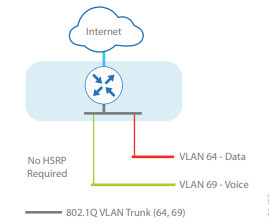
\includegraphics[width=0.5\linewidth]{figure41}}%
%  \subcaptionbox{Another sub-figure\label{fig:rightsubfig}}%
%    {
\includegraphics[width=0.5\linewidth]{knitting-vectorial}}%
  \caption{Topología de Tiendas}
   \textbf{Tomado de:} \textit{autores}.
  \label{fig:fig2subfig}
\end{figure}

La topología WAN de las tiendas es por tanto bastante sencilla, el router en la tienda actuará como un spoke de los dos equipos HBR ubicados en el centro de datos, garantizando de esta manera la integración entre la infraestructura de IWAN y las tiendas.

\section{Diseño de Regionales} % (fold)
\label{sec:Diseño de Regionales}

Las regionales al requerir de mayor ancho de banda, mayor disponibilidad y mayor performance de la red, contarán con dos transportes en el router de borde, de esta forma la tecnología de IWAN realizará el balanceo de carga entre el enlace de internet banda ancha y el enlace MPLS, y contará con redundancia en caso de que alguno de estos enlaces falle.La siguiente imagen muestra de forma general la topología para las regionales.\textbf{Ver figura 10.18 Topología Regionales}.

\begin{figure}[htbp]
  \centering
  %\subcaptionbox{\label{fig:leftsubfig}}%
    {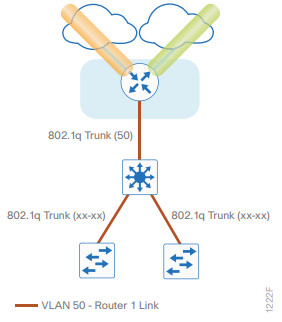
\includegraphics[width=0.5\linewidth]{figure42}}%
%  \subcaptionbox{Another sub-figure\label{fig:rightsubfig}}%
%    {
\includegraphics[width=0.5\linewidth]{knitting-vectorial}}%
  \caption{Topología Regionales}
  \textbf{Tomado de:} \textit{autores}.
  \label{fig:fig2subfig}
\end{figure}

El router formará túneles tanto por internet como por la MPLS hacia el centro de datos y desde allí hacia las demás sedes, en este caso se tendrá una interconexión entre el router de borde y el switch core de la sede, se utilizarán rutas estáticas para alcanzar los diferentes segmentos internos, y estas rutas serán enseñadas al resto de la red mediante el protocolo EIGRP.
\\
\\
En este caso hay redundancia de enlaces ya que el router de borde cuenta con conexión hacia internet y hacia la MPLS por lo que el protocolo PfR se encargará de realizar el balanceo entre los dos enlaces y asegurar la calidad de la voz, video y demás servicios.

\section{Diseño de Sedes Nacionales} % (fold)
\label{sec:Diseño de Sedes Nacionales}

Para el caso de las sedes nacionales debido a su criticidad se requiere no solamente redundancia de enlaces y de fibra sino también de equipos de borde, por lo que la topología cambia para garantizar una mayor disponibilidad en estas sedes. La topología que se tendría en estas sedes es la siguiente: \textbf{Ver figura 10.19 Topología Sedes Nacionales}.

\begin{figure}[htbp]
  \centering
  %\subcaptionbox{\label{fig:leftsubfig}}%
    {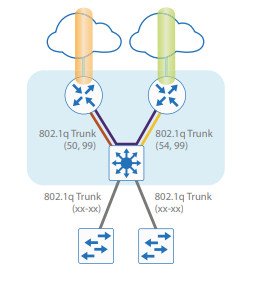
\includegraphics[width=0.5\linewidth]{figure43}}%
%  \subcaptionbox{Another sub-figure\label{fig:rightsubfig}}%
%    {
\includegraphics[width=0.5\linewidth]{knitting-vectorial}}%
  \caption{Topología Sedes Nacionales}
  \textbf{Tomado de:} \textit{autores}.
  \label{fig:fig2subfig}
\end{figure}

En este caso las LAN de los router de borde utilizarían el protocolo HSRP para garantizar la redundancia en caso de presentarse falla sobre alguno de los dos equipos, sin embargo con el fin de asegurar que siga habiendo balanceo de carga entre el enlace de internet y el de MPLS se configura el protocolo EIGRP entre los dos equipos, y se configura uno de los dos routers como branch hub y el otro como spoke con el fin de que PfR siga siendo el responsable de tomar la decisión de por cual de las dos últimas millas se envía el tráfico.

\section{Diseño de Enrutamiento} % (fold)
\label{sec:Diseño de Enrutamiento}


Como se ha mencionado con anterioridad la conectividad entre las sedes se da por medio de túneles GRE multipunto, tecnología también llamada DMVPN, esta es una consideración importante dentro de el diseño de enrutamiento, ya que influye en la decisión de cuál de los protocolos de enrutamiento disponibles son viables para obtener una conectividad escalable y resiliente.
\\
Los protocolos de enrutamiento dinámico considerados para la realización del proyecto fueron los siguientes:

\begin{itemize}
\item[•]\textbf{OSPF}
\item[•]\textbf{EIGRP}
\item[•]\textbf{BGP}
\end{itemize}

El protocolo OSPF es la primera opción en la mayoría de los casos para la conectividad interna del cliente, sin embargo este protocolo de enrutamiento no es recomendado para su utilización con DMVPN debido a su estructura jerárquica. DMVPN tiene una topología Hub and Spoke pero soportando tráfico directamente entre los spokes, aún así esta topología quiere decir que a nivel de enrutamiento todas las sedes deben establecer sus adyacencias a nivel de enrutamiento contra el Hub, con el fin de hacer de DMVPN una topología más escalable se recomienda establecer una sumarización en el Hub de los prefijos de los Spokes, disminuyendo de esta forma la cantidad de espacio de la tabla de enrutamiento y haciendo el enrutamiento más eficiente y más escalable.
\\
\\
Implementar OSPF en una sola área no sería escalable ya que se requerirían enrutadores con muy altas capacidades en cada sede para soportar la tabla topológica completa incluyendo todas las rutas hacia las más de 700 sedes. En inconveniente puntual con OSPF es que dada su naturaleza jerárquica, la sumarización de las rutas puede hacerse únicamente en los ABR, lo cuál implicaría para la topología de DMVPN que cada sede estuviera en un área diferente, lo cuál tampoco escalaría ya que se perderían las ventajas de protocolo de estado de enlace que posee OSPF.
\\
\\
BGP por otro lado es posiblemente el protocolo de enrutamiento existente con la mayor escalabilidad, sin embargo no es muy utilizado como IGP ya que su tiempo de convergencia no es muy alto, con la configuración por defecto de sus temporizadores BGP puede tardar hasta 180 segundos para converger. Por tanto para garantizar un tiempo de convergencia más rápido se excluye este protocolo de enrutamiento de las posibles opciones.
\\
\\
EIGRP por su parte es un protocolo escalable y de rápida convergencia, y en dónde la sumarización puede realizarse en cualquier equipo de la red, por lo que es el protocolo de enrutamiento seleccionado para la solución del cliente. Las adyacencias se realizarían a través de los túneles mGRE y estas se establecerán desde cada una de las sedes remotas contra el router Hub. A continuación se presenta un resumen de cómo se realizan estas adyacencias en EIGRP y la sumarización realizada.

\section{Simulación} % (fold)
\label{sec:Simulación}


Con el fin de definir el comportamiento del diseño planteado se realizaron simulaciones de los dos escenarios, tanto de sedes remotas como de sedes nacionales, para asegurar que la red se comporta tal como se predijo y que se están cumpliendo los requisitos de la disponibilidad y calidad de servicio.

\subsection{Infraestructura Utilizada para la Simulación} % (fold)
\label{sec:Infraestructura Utilizada para la Simulación}

La simulación se realizó utilizando el software GNS3, sin embargo dados los requerimientos de protocolos y dado que se requería de equipos que soporten IWAN no se utilizó GNS3 en su modo tradicional emulando routers directamente en su plataforma, por el contrario se creó una máquina virtual Ubuntu cuyo objetivo es realizar la virtualización de equipos de red, por lo que la simulación fue realizada con VNF creando una máquina virtual para cada uno de los routers simulados, se utiliza por tanto el concepto de virtualización anidada de forma que cada router virtual se crea como una máquina virtual dentro de otra máquina virtual, el esquema de esta virtualización \textbf{Ver figura 10.20 Infraestructura Utilizada para la Simulación}.
\begin{figure}[htbp]
  \centering
  %\subcaptionbox{\label{fig:leftsubfig}}%
    {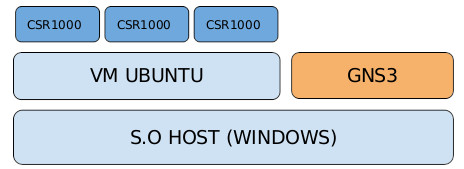
\includegraphics[width=0.7\linewidth]{figure44}}%
%  \subcaptionbox{Another sub-figure\label{fig:rightsubfig}}%
%    {
\includegraphics[width=0.5\linewidth]{knitting-vectorial}}%
  \caption{Infraestructura Utilizada para la Simulación}
  \textbf{Tomado de:} \textit{autores}.
  \label{fig:fig2subfig}
\end{figure}
Esta virtualización Anidada se realizó utilizando VMware workstation pro, mediante esta herramienta se virtualizó la VM de Ubuntu dentro del sistema operativo Windows, a su vez dentro de esta máquina virtual de Ubuntu se utilizó virtualización KVM para montar cada uno de los enrutadores virtuales.
\\
\\
Esta configuración permite por un lado mantener contenidos dentro de la máquina virtual Ubuntu los recursos que utilizan los enrutadores virtuales de manera que la utilización de estas máquinas no colapse el sistema operativo host al dejar sin recursos el sistema operativo y permite por otro lado integrar GNS3 con routers VNF reales, en este caso los CSR1000v de Cisco que están diseñados específicamente para servicios en la nube y soportan todas las características requeridas por la solución de IWAN. Estos enrutadores virtuales requieren 1 core y 3GB de RAM, por tanto la simulación se realizó en un equipo con las siguientes carácteristicas técnicas \textbf{tabla 10.12 Caracteríticas Técnicas}:

\begin{table}[ht]
	\caption{Caracteríticas Técnicas}
	\label{tab:hla:results}
\centering
\begin{tabular}{lccccc}
	\toprule
	\multicolumn{1}{c}{\textbf{Dipositivo}} 	& \textbf{Recursos}\\
	\midrule
\cite{Memoria RAM} 		& 16 GB \\
\cite{CPU} 		& intel core i7 7700HQ - 4 cores \\
\cite{Disco Duro} 		& 1T HD + 128GB SSD \\
	\midrule
	\textbf{Total}			& \textbf{--} \\
	\bottomrule
\end{tabular}
\end{table}

De estos recursos tuvieron que asignarse 12MB de memoria RAM para la máquina virtual ya que cada uno de los routers requiere 3MB de Memoria para funcionar correctamente y 4 threads de procesamiento de los 8 disponibles para el procesamiento requerido por los enrutadores, por otra lado solamente 8GB de disco duro fueron suficientes para esta máquina virtual.

\subsection{Topologías y Configuraciones Realizadas} % (fold)
\label{sec:Topologías y Configuraciones Realizadas}

Dado el diseño planteado se realizaron pruebas con dos topologías diferentes, la primera siendo la topología de las sedes nacionales, es decir dos CPE en la sede cada uno recibiendo un hilo de fibra por un transporte diferente. Para esta topología se incluyeron un total de 5 enrutadores, dos realizando la función de HBR (Hub Border Router) que actúan como Hubs para los túneles en la topología DMVPN y un MC(Master Controller) encargado de establecer las políticas de PfR de cada una de las aplicaciones y propagar las políticas por el resto de la red.\textbf{Ver figura 10.21 La topología configurada en GNS3}.
\begin{figure}[htbp]
  \centering
  %\subcaptionbox{\label{fig:leftsubfig}}%
    {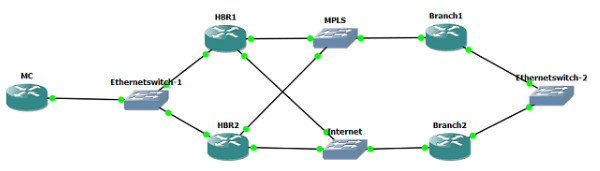
\includegraphics[width=0.9\linewidth]{figure45}}%
%  \subcaptionbox{Another sub-figure\label{fig:rightsubfig}}%
%    {
\includegraphics[width=0.5\linewidth]{knitting-vectorial}}%
  \caption{La topología configurada en GNS3}
  \textbf{Tomado de:} \textit{autores}.
  \label{fig:fig2subfig}
\end{figure}

En la topología se simulan los diferentes transportes con switches, uno para la MPLS y otro para el transporte de internet, esto es una simplificación de las redes de transporte reales ya que estas son mucho más complejas, pero en este caso la simulación mantiene su validez ya que para establecer los túneles que funcionan acá como la red “underlay” únicamente se requiere conectividad IP entre los routers Branch y los HBR sin importar la forma como esta se de.

Como se mencionó anteriormente los HBR actúan como Hubs para la topología DMVPN y en esta topología los dos equipos Branch se registran contra dichos equipos como lo muestra \textbf{Ver figura 10.22 Branch1} para el Branch1 y \textbf{Ver figura 10.24 Branch2} para el Branch2

\begin{figure}[htbp]
  \centering
  %\subcaptionbox{\label{fig:leftsubfig}}%
    {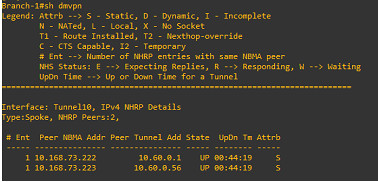
\includegraphics[width=0.7\linewidth]{figure46}}%
%  \subcaptionbox{Another sub-figure\label{fig:rightsubfig}}%
%    {
\includegraphics[width=0.5\linewidth]{knitting-vectorial}}%
  \caption{Branch1}
  \textbf{Tomado de:} \textit{autores}.
  \label{fig:fig2subfig}
\end{figure}


\begin{figure}[htbp]
  \centering
  %\subcaptionbox{\label{fig:leftsubfig}}%
    {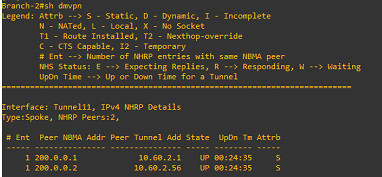
\includegraphics[width=0.7\linewidth]{figure47}}%
%  \subcaptionbox{Another sub-figure\label{fig:rightsubfig}}%
%    {
\includegraphics[width=0.5\linewidth]{knitting-vectorial}}%
  \caption{Branch2}
  \textbf{Tomado de:} \textit{autores}.
  \label{fig:fig2subfig}
\end{figure}

Además de estas adyacencias de DMVPN se configuró EIGRP como protocolo de enrutamiento utilizado tanto hacia los túneles como entre los routers Branch y en datacenter entre los HBR y el MC, las \textbf{Ver figura 10.25 Configuración EIGRP} y \textbf{Ver figura 10.26 Configuración EIGRP} muestran los establecimientos de dichas adyacencias en el Branch.

\begin{figure}[htbp]
  \centering
  %\subcaptionbox{\label{fig:leftsubfig}}%
    {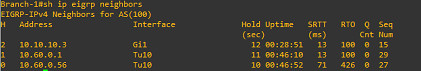
\includegraphics[width=0.7\linewidth]{figure48}}%
%  \subcaptionbox{Another sub-figure\label{fig:rightsubfig}}%
%    {
\includegraphics[width=0.5\linewidth]{knitting-vectorial}}%
  \caption{Configuración EIGRP}
  \textbf{Tomado de:} \textit{autores}.
  \label{fig:fig2subfig}
\end{figure}


\begin{figure}[htbp]
  \centering
  %\subcaptionbox{\label{fig:leftsubfig}}%
    {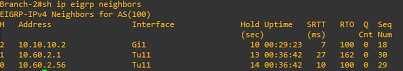
\includegraphics[width=0.7\linewidth]{figure49}}%
%  \subcaptionbox{Another sub-figure\label{fig:rightsubfig}}%
%    {
\includegraphics[width=0.5\linewidth]{knitting-vectorial}}%
  \caption{Configuración EIGRP}
  \textbf{Tomado de:} \textit{autores}.
  \label{fig:fig2subfig}
\end{figure}

Finalmente el otro componente que hace parte de la solución de IWAN es PfR, en este caso uno de los routers (El activo en la configuración de HSRP) toma el rol de master en PFR encargándose de distribuir las políticas a los border router del Branch, las imagenes \textbf{Ver figura 10.27 Registros de los Routers}y \textbf{Ver figura 10.28 Registros de los Routers} muestran el registro de los dos routers con PfR.

\begin{figure}[htbp]
  \centering
  %\subcaptionbox{\label{fig:leftsubfig}}%
    {\includegraphics[width=0.5\linewidth]{figure50}}%
%  \subcaptionbox{Another sub-figure\label{fig:rightsubfig}}%
%    {\includegraphics[width=0.5\linewidth]{knitting-vectorial}}%
  \caption{Registros de los Routers}
  \textbf{Tomado de:} \textit{autores}.
  \label{fig:fig2subfig}
\end{figure}


\begin{figure}[htbp]
  \centering
  %\subcaptionbox{\label{fig:leftsubfig}}%
    {\includegraphics[width=0.5\linewidth]{figure51}}%
%  \subcaptionbox{Another sub-figure\label{fig:rightsubfig}}%
%    {\includegraphics[width=0.5\linewidth]{knitting-vectorial}}%
  \caption{Registros de los Routers}
  \textbf{Tomado de:} \textit{autores}.
  \label{fig:fig2subfig}
\end{figure}

El diseño para las sedes regionales difiere de las sedes nacionales en cuanto a que por costos no se utilizan dos routers sino uno sólo con dos métodos de transporte independientes, en este sentido la distribución y configuración de la topología en datacenter se mantiene exactamente igual, el único cambio de configuración se realiza sobre el router Branch, la topología simulada para este caso es ilustrada en la figura \textbf{Ver figura 10.29 Topología Router Branch}

\begin{figure}[htbp]
  \centering
  %\subcaptionbox{\label{fig:leftsubfig}}%
    {\includegraphics[width=0.9\linewidth]{figure52}}%
%  \subcaptionbox{Another sub-figure\label{fig:rightsubfig}}%
%    {\includegraphics[width=0.5\linewidth]{knitting-vectorial}}%
  \caption{Topología Router Branch}
  \textbf{Tomado de:} \textit{autores}.
  \label{fig:fig2subfig}
\end{figure}

En este caso el único router branch contará con 4 adyacencias de DMVPN, dos por cada HBR, correspondientes a los diferentes tipos de transporte. Esto asegura que hay redundancia en caso de que alguno de los HBR falle o en caso de ruptura de fibra óptica para alguno de los canales de transporte. la imagen \textbf{Ver figura 10.30 Registro desde el Router} ilustra la forma como se ve este registro desde el router.

\begin{figure}[htbp]
  \centering
  %\subcaptionbox{\label{fig:leftsubfig}}%
    {\includegraphics[width=0.6\linewidth]{figure53}}%
%  \subcaptionbox{Another sub-figure\label{fig:rightsubfig}}%
%    {\includegraphics[width=0.5\linewidth]{knitting-vectorial}}%
  \caption{  Registro desde el Router}
  \textbf{Tomado de:} \textit{autores}.
  \label{fig:fig2subfig}
\end{figure}

De igual forma a pesar de que se forman adyacencias EIGRP por los túneles GRE multipunto únicamente contra los 2 HBR se establecen 4 vecindades de HSRP diferentes, dos por cada HBR, este comportamiento puede verse más claramente en el router como lo muestra la figura \textbf{Ver figura 10.31 Adyacencias EIGRP por los Túneles GRE}

\begin{figure}[htbp]
  \centering
  %\subcaptionbox{\label{fig:leftsubfig}}%
    {\includegraphics[width=0.5\linewidth]{figure54}}%
%  \subcaptionbox{Another sub-figure\label{fig:rightsubfig}}%
%    {\includegraphics[width=0.5\linewidth]{knitting-vectorial}}%
  \caption{  Adyacencias EIGRP por los Túneles GRE}
  \textbf{Tomado de:} \textit{autores}.
  \label{fig:fig2subfig}
\end{figure}

En cuanto al protocolo PfR el mismo router cumple las funciones de master y de borde para el branch, registrándose y descargando las políticas desde el MC en el datacenter. La imagen \textbf{Ver figura 10.32  Protocolo PfR} muestra dicho registro.

\begin{figure}[htbp]
  \centering
  %\subcaptionbox{\label{fig:leftsubfig}}%
    {\includegraphics[width=0.5\linewidth]{figure55}}%
%  \subcaptionbox{Another sub-figure\label{fig:rightsubfig}}%
%    {\includegraphics[width=0.5\linewidth]{knitting-vectorial}}%
  \caption{  Protocolo PfR}
  \textbf{Tomado de:} \textit{autores}.
  \label{fig:fig2subfig}
\end{figure}
